 \documentclass{article}

\usepackage{graphicx}
\usepackage[toc,page]{appendix}

\usepackage[a4paper]{geometry}
\usepackage[english]{babel}
\usepackage[T1]{fontenc}
\usepackage{hyperref}
\usepackage{amstext,amsmath,amsfonts}
\usepackage{dcolumn,booktabs}
\usepackage{color}
\usepackage{subfigure}
\usepackage{amsthm}

\makeatletter
\def\maketitle{%
  \null
  \thispagestyle{empty}%
  \vfill
  \begin{center}\leavevmode
    \normalfont
    {\LARGE \@title\par}%
    \vskip 1cm
    {\Large \@author\par}%
    \vskip 1cm
    {\Large \@date\par}%
  \end{center}%
  \vfill
  \null
  \cleardoublepage
  }
\makeatother
\title{On nonlinearities in stock prices: an intrinsic bubble approach}

\author{Kees ter Brugge\\}
                
                
\date{\today}

\begin{document}
 \maketitle



\newpage
\section{introduction}

Economists have always tried to understand and make predictions about the financial markets. The efficient market hypothesis states that the law of supply and demand adjusts stock prices so that they reflect all information available to the market. This means that a stock's price is equal to its fundamental value. The present-value model gets much attention from economists and argues that a stock's fundamental value is equal to its expected discounted future dividends. There is an considerable body of empirical evidence against the present-value model. Leroy and Porter (1981) and Shiller (1981) show that actual stock prices are much more volatile than the predictions made by the present-value model and that the prediction of a constant price-dividend ratio is not consistent with observed ratio's. Economists have tried to explain this excessive volatility by attributing it to variable discount rates (West(1987, 1988), Campbell and Shiller(1988b)), Noise traders (DeLong, Shleifer, Summers and Waldmann(1990)), fads (Shiller (1981)) and regime switching in the dividend process (Driffill and Sola(1998)) 

Another approach to explaining the observed volatility is by including a rational bubble in the present-value model. This approach is fueled by the boom and bust periods that have occured throughout history, for example in 1929, 1987 and 2000 with U.S. stock prices or more recently the credit crisis. One category of proposed rational bubbles are the speculative bubbles which are driven by self-fulfilling prophecies. They are consistent with Keynes's (1936) idea that investors pay less attention to market fundamentals than to what they expect the average opinion to expect about the average opinion. These bubbles (see Evans (1991), Schaller and Norden (2002)) are exogenous to economic fundamentals and grow exponentially. They have a growing probability of bursting relative to their size, such that they do not violate the no-arbitrage principle. The results from these researches are often in conflict with each other and are inconclusive(G�rkaynak (2008)). Usually the no bubble hypothesis is rejected, which is the same as rejecting the present-value model. The problem with these methodologies is that it is never clear whether the rejection can be attributed to the existence of their bubble specification or to a misspecification of the present-value model.

Many economist found the attribution of observed price behaviour left unexplained by the present-value model to unobservable outside forces not satisfying and wanted a model in which only market fundamentals provided the epxlanation.Froot and Obstfeld (1991) introduced such a bubble specification, namely the intrinsic bubble. Intrinsic bubbles are deterministic nonlinear functions of dividends, so they are only determined by market fundamentals and therefore endogenous. 

Driffill and Sola (1998) show that if dividends are assumed to be a markov regime-switching process, the inclusion of an intrinsic bubble does not add not much explanatory value. This result is consistent with  Flood and Garber's (1980) and Flood and Hodrick's (1986) finding that when investigating the failure of the present-value model, it is not possible to distinguish between changes in the processes driving market fundamentals and the presence of rational bubbles as  the cause for the failure. 

But intrinsic bubbles seem compelling. They are parsimonious because they do not introduce new variables. Furthermore, 
they allow stable periods of deviations from the price predicted by the present-value model and reproduce the ineffiecient overreaction of prices to changes in fundamentals. Intrinsic bubbles are consistent with the finding of Kanas (2005) that the failure of the present-value model might be due to the relation of prices and dividends being nonlinear instead of linear.

With this paper we extend the papers of Froot and Obstfeld's (1991) and Ma and Kanas's (2004) who rejected the absence of an intrinsic bubble  in the S\&P 500 and rejected the existence of a linear long-run relation of prices and dividends.

%what about to do in my thesis
The first part of this paper shows how an intrinsic bubble fits into the present-value model and presents its properties. In the second part the Standard \& Poor's 500 index is used to  show where the present-value model fails in explaining price behaviour and test whether the intrinsic bubble model provides more explanatory power. Froot and Obstfelds's (1991) work is extended in that a time series is used that includes recent extreme price behaviour and the possibility that using a subsample provides a more accurate model is explored. Ma and Kanas (2004 ) use Granger and Hallman's (1991) nonlinear cointegration test to test for a long-run nonlinear relationship of prices and dividends. In this paper Breitung's (2001) rank-based cointegration is used, since he showed that such residual-based tests are inconsistent for some classes of nonlinear functions. In the third part we discuss the results and compare them with findings of others to see if different testing methods or recent events have changed the results.

The appendix contains an explanation of the nonlinear least squares regression and a simulation to assess its accuracy. Furthermore, it contains the R codes that are used to produce some of the results in this paper. Most of the results are obtained using Eviews 5.

\newpage

\section{The model}

An often used model to valuate assets is a simplified version of the model Lucas (1978) suggests. In this model, there are a large number of infinitely lived and identical agents. We assume these agents to be risk neutral. This gives us the following stochastic difference equation for equilibrium prices
\begin{eqnarray}
P_t = e^{-r} E_t(D_t + P_{t+1}) \label{standard}
\end{eqnarray}
where $P_t$ is the real stock price at the beginning of period $t$, $D_t $ are the real dividends per share paid over period $t$ and $E_t$ is the mathematical expectation conditioned on information available at the beginning of period $t$. $e^{-r}$ is the discount rate, where $r $ is the constant, continuous real rate of interest. 

Equation (\ref{standard}) has multiple solutions. A particular one is the present-value solution $P_t^{pv}$, which is obtained by iterating and using the law of iterated expectation:
\begin{eqnarray}
P_t^{pv} &=& e^{-r} E_t(D_t) +  e^{-r} E_t(P_{t+1}) = e^{-r} E_t(D_t) +  e^{-r}E_t(e^{-r} E_{t+1}(D_{t+1} + P_{t+2}))  \notag \\
&=& e^{-r} E_t(D_t) + e^{-2r} E_{t}(D_{t+1}) + e^{-2r}E_t(e^{-r} E_{t+2}(D_{t+2} + P_{t+3})) \notag \\
&=& e^{-r} E_t(D_t) + e^{-2r} E_{t}(D_{t+1}) + e^{-3r}E_t(D_{t+2}) + \cdots \notag \\
&=& \sum_{s=0}^{\infty}e^{-(s+1)r}E_t(D_{t+s}) \label{present-value}
\end{eqnarray}
if we assume
\begin{eqnarray}
\lim_{s\rightarrow \infty} e^{-rs}E_t(P_s) = 0 \label{transversality}
\end{eqnarray}
Condition (\ref{transversality})is known as the transversality condition and can be interpretated as assuming that the present value of an asset at time infinity is zero. This rules out the possibility of infinitely lived agents holding on to their stocks for infinity. The present-value solution equates a stock's price to its discounted expected future payments. We assume the continuously compounded growth rate of expected dividends to be smaller than $r$, so that the present-value solution does not diverge and therefore always exists.

Another group of solutions to (\ref{standard}) is obtained by adding a rational bubble component
\begin{eqnarray}
P_t = P_t^{pv} + B_t \label{sum}
\end{eqnarray}
where 
\begin{eqnarray}
B_t = e^{-r}E_t(B_{t+1}) \label{rational}
\end{eqnarray}
These solutions violate condition (\ref{transversality})
unless the bubble component is equal to zero. Condition (\ref{rational}) excludes arbitrage oppurtunities.

\subsection{Properties of an intrinsic bubble}
Froot and Obstfeld (1991) claim that the component of prices left unexplained by the present-value model is highly positively correlated with dividends. They suggest an 'intrinsic' bubble that only depends on fundamentals and not on extraneous factors. To find the function of this bubble, assumptions about the stochastic process for dividends $D_t$ have to be made. A common assumption is that log dividends, $d_t$, is a random walk \footnotemark with constant drift $\mu$
\footnotetext{Froot and Obstfeld (1991) argue that a random walk is a plausible approximation to the mechanism the market uses to forecast dividends (see appendix A, p. 1209)}
\begin{eqnarray}
d_{t+1} = \mu + d_t + \xi_{t+1} \label{lognormal}
\end{eqnarray}
where $\xi_{t+1}$ is a normal random variable with conditional mean zero and variance $\sigma^2$. If we additionally assume $D_t$ to be known at the beginning of period $t$ and 
\begin{eqnarray}
P_t^{pv} &=&  \sum_{s=0}^{\infty}e^{-(s+1)r}E_t(D_{t+s}) = \sum_{s=0}^{\infty}e^{-(s+1)r}E_t(e^{d_{t+s}}) = \sum_{s=0}^{\infty}e^{-(s+1)r}E_t(e^{d_t + s\mu + \sum_{i=1}^{s} \xi_{t+i}}) \notag \\
 &=& D_t e^{-r} \sum_{s=0}^{\infty} e^{-sr + s\mu + \frac{s\sigma^2}{2}} = D_t e^{-r} \sum_{s=0}^{\infty} \left(e^{-r + \mu + \frac{\sigma^2}{2}}\right)^s
 = D_t e^{-r} \frac{1}{1 - e^{-r + \mu + \frac{\sigma^2}{2}}} \notag \\ 
 &=& D_t \frac{1}{e^r - e^{\mu + \frac{\sigma^2}{2}}} = D_t \kappa \label{kappa}
\end{eqnarray}
since $E_t(e^{\xi_{t+1}}) = e^{\frac{\sigma^2}{2}}$.  $\kappa$ represents the inverse of the required rate of return on stocks less the expected rate of growth of dividends and is equal to the ratio of the present-value price and dividends. It is defined as follows
\begin{eqnarray}
\kappa = \frac{1}{e^r - e^{\mu + \frac{\sigma^2}{2}}}  \label{eqkappa}
\end{eqnarray}
 The sum in (\ref{kappa})converges because we have assumed the continuously compounded growth rate of expected dividends to be smaller than $r$,
\begin{eqnarray}
r > \mu + \frac{\sigma^2}{2} \label{grow} 
\end{eqnarray}
to ensure the existence of the present-value solution.

The bubble proposed by Froot and Obstfeld is a nonlinear function of current dividends
\begin{eqnarray}
B(D_t) = cD_t^\lambda \label{intrinsic}
\end{eqnarray}
which satisfies condition (\ref{rational}) if the following condition holds
\begin{eqnarray}
\lambda = \frac{\sqrt{\mu^2 + 2r\sigma^2} - \mu}{\sigma^2} \label{eqlambda}
\end{eqnarray}
because then
\begin{eqnarray}
e^{-r}E_t(B(D_{t+1})) &=& e^{-r}E_t(cD_{t+1}^{\lambda}) = e^{-r}E_t(ce^{d_{t+1}\lambda}) = e^{-r}E_t(ce^{(\mu + d_t + \xi_{t + 1})\lambda}) \notag \\ 
 &=&  ce^{d_t\lambda}e^{-r + \lambda \mu }E_t(e^{\xi_{t+1}\lambda} = cD_t^{\lambda}e^{-r + \lambda \mu + \frac{\lambda^2 \sigma^2}{2}} = cD_t^{\lambda} = B(D_t) \notag
\end{eqnarray}
 We choose $\lambda$ to be the positive root of the equation, because we want the size of the bubble to go to zero as dividends go to zero. This together with condition (\ref{grow}) implies $\lambda > 1$. $c$ is a nonnegative constant, because stock prices cannot be negative. It would violate free disposability.
Now we can rewrite (\ref{sum}) so that it includes an intrinsic bubble, obtaining our intrinsic bubble model.
\begin{eqnarray}
P_t = P_t^{pv} + B(D_t) = \kappa D_t + c D_t^{\lambda} \label{sumintrinsic}
\end{eqnarray}
When $\lambda$ is near one this model can suffer from colinearity. Therefore it is better to use the price-dividend ratio model 
\begin{eqnarray}
\frac{P_t}{D_t} =  \kappa  + c D_t^{\lambda - 1} \label{sumratio}
\end{eqnarray}
While the present-value solution suggests a constant price-dividend ratio $\kappa$, the inclusion of an intrinsic bubble implies that the ratio is a function of dividends. 


\section{Application to Standard \&Poor's 500}


\begin{figure}[h!]
	\centering
		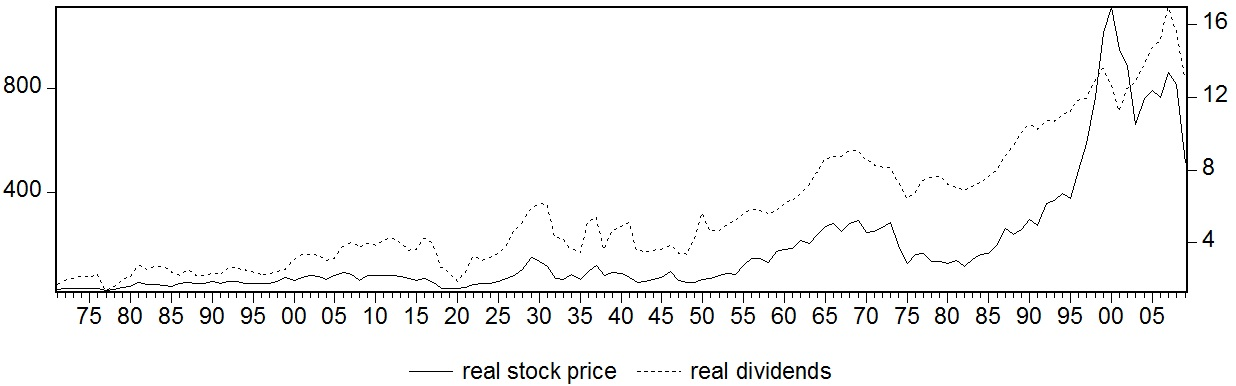
\includegraphics[width=0.99\textwidth]{C:/Users/kc/Downloads/divandprice.jpg}
	\caption{Plot of real dividends $D_t$ and real prices $P_t$ over 1871 - 2009. The left axis scales the prices and the right axis scales the dividends.}
	\label{pricediv}
\end{figure}

%decribe, plot data, show linear when logtransformed and stationary when differenced hence integrated order one.
To examine the validity of the models we defined before, we use data on the U.S. stock market from 1871 untill 2009. The used stockprice index is the January values of the Standard and Poor's Composite annual stock price index. The time series is an updated version of the often used data from Shiller (1989). Since data on January values of the dividends index are not available, we use annual averages for the calendar year, following Froot and Obstfeld (1991). They found that this does not affect results statistically\footnotemark. Stock prices and dividends are deflated by the Produces Price Index of 1982. \footnotetext{see Froot and Obstfeld (1991) footnote 18, p. 1198} We use data till 2006 to estimate the coefficients, so that we can perform out-of-sample forecasts which we can compare with the last three realizations. 
The Standard and Poor's composite index is considered as one of the best benchmarks of U.S. stock market performance. It is a market value weighted index that includes 500 stocks that trade on either the New York Stock Exchange and the NASDAQ. The selection of stocks is mostly based on market size, liquidity and sector. The S$\&$P monthly index series was created in 1957 and is extended back to January 1871 by Cowles. 
\

In figure (\ref{pricediv}) we see that dividends and prices seem to have an exponential trend. To assess the nature of these processes, we want to produce stationary series. In figure (\ref{lnpricediv}) the log transformation of both series is shown. The series seem to have a linear trend now. The series move together, which indicates correlation of the series. Furthermore, their trend also seems equally steep, which suggests that these processes might be cointegrated.


\begin{figure}[t!]
	\centering	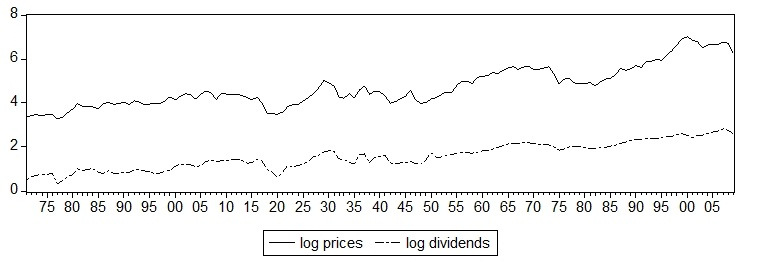
\includegraphics[width=0.9\textwidth]{C:/Users/kc/Downloads/logpricediv.jpg}
	\caption{Plot of $d_t$ and $p_t$ with sample period 1871 - 2009}
	\label{lnpricediv}
\end{figure}

In figure (\ref{dlnpricediv}) the first difference of the log transformation of prices and dividends is plotted. The series appear to be stationary. This suggests that log dividends,$d_t$, and log prices, $p_t$, are integrated of order one. 

\begin{figure}[h!]
	\centering
		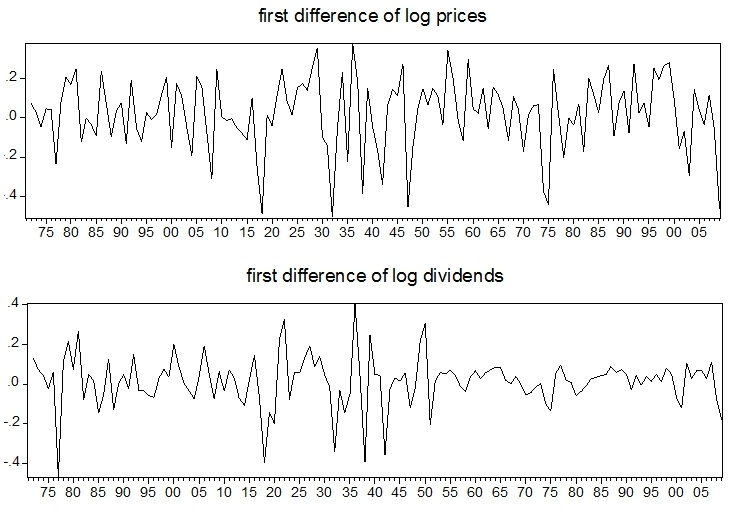
\includegraphics[width=0.7\textwidth]{C:/Users/kc/Downloads/dlogdivprice.jpg}
	\caption{Plot of $\Delta d_t$ and $\Delta p_t$ with sample period 1872 - 2009}
	\label{dlnpricediv}
\end{figure}

If we look at figure (\ref{dlnpricediv}) we see that after 1955 the first-difference series of log dividends, $\Delta d_t$, is less volatile than before 1955. We have a sample period of 139 years. In this time changes in fundamental could have occurred. Since dividends is the explanatory variable of our model it is a good idea to estimate the model using a subsample with 1955 as starting date in addition to using the whole sample.	 This could give us better estimates, which in turn leads to a better assessment of the statistical significance of the model and more accurate forecasts. 

Fo be able to evaluate the forecasting performance of the model, the available data set is dividend into two subsamples. The first subsample contains the data from 1871 till 2006. This estimations subsample is used to estimate the model. We call the last three observations the forecasting subsample.
\newpage
	
To be able to execute some tests on the intrinsic bubble model we have to assume that the error  term $\eta_t$ we add to (\ref{sumratio}) to get
\begin{eqnarray}
\frac{P_t}{D_t} =  c_0  + c D_t^{\lambda - 1} + \eta_t \label{intrinsicmodel}
\end{eqnarray}
is well-behaved, meaning that $\eta_t$ is statistically independent of dividends at all leads and lags and has unconditional mean zero\footnotemark. Otherwise the statistical tools we use do not lead to unbiased estimates. $\eta_t$ can be interpreted as any shock to the price-dividend ratio that has no predictive power with respect to future dividens, such as fads. 
%hier regressie van eta op epsilonsss
\footnotetext{Froot and Obstfeld (1991) also made these assumptions. For a justification see footnote 16, p. 1198}

The no bubble hypothesis corresponding to this model is that $c_0 = \kappa$ and $c=0$, meaning that the present-value model is true, so that the level of dividends has no impact on the price-dividend ratio. The alternative hypothesis is that there is a bubble involved, a relation between dividends and the price-dividend ratio, implying $c_0 = \kappa$ and $c > 0$. 

The values of $\kappa$ and $\lambda$ implied by the properties of the intrinsic bubble model, $\overline{\kappa}$ and $\overline{\lambda}$, are obtained using the estimates of  $\mu, \sigma$ and $r$ in equations (\ref{eqkappa}) and (\ref{eqlambda})\footnotemark \footnotetext{ We obtain the continuous interest rate as follows  $\overline{r} = log(\frac{\sum_{t=m}^{2005}\frac{P_{t+1} + D_t}{P_t}}{2005-m})$, where $m$ is $1871$ for the estimate based one the whole sample and  $1955$ based on the subsample.}. The estimates are reported in table (\ref{point}). 
\begin{table}[h!]
\centering
\begin{tabular}{l | l l  }
\hline \\
parameter & whole sample 1871 - 2006 & subsample 1955 - 2006\\ \hline 
$r$  & 0.0904 & 0.1009 \\
$\mu$ & 0.0162 & 0.0204\\
$\sigma$ & 0.1257 & 0.0544 \\
$\kappa$ & 14.2411 & 11.8984 \\
${\lambda}$ & 2.5094 &  3.8634 \\
\end{tabular}
\caption{Estimates of parameters for the two samples}
\label{point}
\end{table}

In figure (\ref{lnpricediv}) we clearly see that log dividends has a positive trend. Using the estimates reported in the table above we can calculate that under the assumption that log dividends has no trend, the p-value of the estimate of $\mu$ is equal to 0.14 for the whole sample and 0.01 for the subsample. These statistics support the perceived break in the dividends process.
We can also see that the subsample predicts a bubble that is more explosive than the one predicted by the whole sample.


\subsection{The failure of the present-value model}
The present-value model (\ref{present-value}) predicts that the following regression 
\begin{eqnarray}
P_t = \beta_0 + \beta D_t  + v_t \label{regpv}
\end{eqnarray}
gives us an estimate of $\beta$ that is close to $\overline{\kappa}$. When we perform an regression on the log transformations of prices and dividends instead 
\begin{eqnarray}
p_t = \beta_0 + \beta d_t  + v_t \label{reglnpv}
\end{eqnarray}
we expect to find an estimate of $\beta$ near one, since the linear relation between prices and dividends implied by the present-value model has an elasticity equal to one. \\

On the other hand, if (\ref{intrinsicmodel}) is true, the estimate of $\beta$ we expect to find from regressing (\ref{regpv})  is much bigger than $\overline{\kappa}$, since the derivative of prices with respect to dividends predicted by the intrinsic model contains an additional positive nonlinear component, $\frac{d B_t}{d D_t}  = \lambda c D_t^{\lambda - 1}$, compared to the derivative predicted by the present-value model.
Furthermore, (\ref{intrinsicmodel}) implies a nonlinear relation between $P_t$ and $D_t$ and since $\lambda$ is bigger than one, this relation has an explosive nature. The estimate of $\beta$ that follows from regressing (\ref{reglnpv}) should be bigger than one. Prices would appear to overreact to changes in dividends. 
\
\begin{table}[h!]
\centering
\begin{tabular}{l | l | l l l l }
\hline \\
regression equation & $\beta$ whole sample & $\beta$ subsample \\
\hline \\
 $P_t = \beta_0 + \beta D_t  + v_t$ &  56.0023 & 89.2800 \\
$p_t = \beta_0 + \beta d_t  + v_t$ & 1.4475 & 2.1273   \\ \hline 
\end{tabular}
\caption{results of OLS regressions.}
\label{sensitivity}
\end{table}

When we compare table (\ref{sensitivity}) and table (\ref{point}) we see that the estimates of $\beta$ are much higher than those predicted by the present-value model.

\begin{figure}[h!]
	\centering
		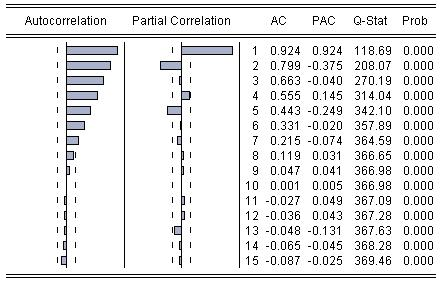
\includegraphics[width=0.6\textwidth]{C:/Users/kc/Downloads/1871pvcorrelo.JPG}
	\caption{correlogram of $v_t$ resulting from regression $P_t = \beta_0 + \beta D_t  + v_t$ with sample period 1871 - 2006. }
	\label{correlo}
\end{figure}

In figure (\ref{correlo}) we see the correlogram resulting from regressing the present-value model (\ref{regpv}). These results are similar for the subsample. The residuals have a lot of positive autocorrelation. This model is not able to produce white noise residuals.  


Another way to assess the validity of the present-value model is to test for cointegration. Cointegration indicates a long-run relationship between two or more series. As can be seen in figure (\ref{dlnpricediv}) log prices and log dividends seem to be integrated of order one, since their first difference is stationary. The Phillips-Perron unit root test with intercept gives us the adjusted t-staticstics -0.64 and  -0.68 for the whole sample and -1.13 and -0.55 for the subsample for log prices and log dividends respectively. That means that the hypothesis that these processes have a unit root is not rejected for any reasonable significance level. It is common to assume that an exponontial transformation of an series that is integrated of order one is also integrated of order one, so from here on we assume that prices and dividends are also integrated of order one. We do not test for a unit root in prices and dividends using the Phillips-Perron test, since it lacks power when testing a series with a nonstationary first-difference.  Under the present-value model prices and dividends, and log prices and log dividends should be linearly cointegrated.

\begin{table}[h!]
\centering
\begin{tabular}{l | l l }
\hline \\
Variables used in test for cointegration & whole sample & subsample \\
\hline \\
$P_t$ and $D_t$ & 11.7263 & 11.6657 \\ 
$p_t$ and $d_t$ & 7.6584 & 6.8591  \\
\hline 
\end{tabular}
\caption{The reported values are the unrestricted cointegration rank test trace statistics obtained by the Johansen methodology under the null hypothesis of no cointegration, where * denotes statistical significance at the 5 \% level.}
We see in the table above that the hypothesis of no cointegration is not rejected for all of the tests. \\
Under the present-value model the price-dividend ratio should be constant. We see however in the figure below that a constant fits the price-dividend ratio really bad. The greatest estimate of $\kappa$, made by the whole sample, is added to the figure to illustrate the fact that the price-dividend ratio in the S\&P 500 is consistently much greater than predicted by the present-value model. Furthermore, the ratio is nonstationary, which is not expected under the present-value model. 
\end{table}

\begin{figure}[h!]
\centering
		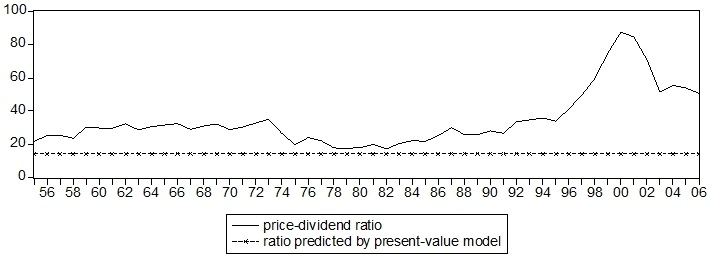
\includegraphics[width=0.99\textwidth]{C:/Users/kc/Downloads/ratio1.jpg}
	\label{ratio}
\end{figure}



There are a few problems with the present-value model. Prices are too sensitive to dividends and seem to have an elasticity  to dividends greater than one, suggesting  a nonlinear relation. The price-dividend ratio is not stationary and is too high given the rate of return. Futhermore, there seems to be no evidence supporting a linear long-run relation between prices and dividends. The present-value model also produces highly autocorrelated residuals.

The intrinsic bubble model seems to have the potential to solve these problems.  

\subsection{The intrinsic bubble model}


To see if a nonlinear function of dividends explains the variation in prices and the nonstationarity in  price-dividend ratios better than the present-value model, we estimate (\ref{intrinsicmodel}) using the nonlinear least squares method\footnotemark \footnotetext{For an explanation of the method, see appendix A}.  Even though the intrinsic bubble model(\ref{intrinsicmodel}) contains an nonlinear regressor, the estimates of the coefficients approximate a normal distribution\footnotemark \footnotetext{See appendix B for a simulation}. We already assumed that the $\eta_t$ are identically distributed, independent of dividends at all leads and lags and have unconditional mean zero. The standard t-statistic approximates a normal distribution under these conditions \footnotemark. \footnotetext{see Froot and Obstfeld (1991), Appendix B}

Since we have not assumed that $\eta_t$ is distributed independently, the residuals may be serially correlated. This can lead to incorrect estimations of the standard errors of coefficients. To counteract this, we correct the residuals using Newey and West's (1987) covariance matrix estimator.




\begin{table}[h]
\centering
\begin{tabular}{l|l | l l l l l l l}
\hline \\
sample & estimated model & $ c_0 $ & $ c $ & $\lambda$ & $ F stat.$ & $R^2$  & ln(L)\\
\hline \\
1871 - 2006&$ \frac{P_t}{D_t} =  c_0  + c D_t^{\lambda - 1} + \eta_t $ & 17.9962 & 0.0413 & 3.6420 & 26.79 *** & 0.69 & -460.44 \\
& & (12.06)** & (0.58) & (5.37)** & & &\\
1955 - 2006&$ \frac{P_t}{D_t} =  c_0  + c D_t^{\lambda - 1} + \eta_t $ & 12.6979 & 0.2269 & 3.0345 & 17.66 *** & 0.59 &-195.84 \\
& & (0.75) & (0.23) & (1.95) & & &\\
1871 - 2006 & $  \frac{P_t}{D_t} =  c_0  + c D_t^{2.5094 - 1} + \eta_t $ & 13.5220 & 0.7684 & & & 0.64 & -470.47  \\
& & (8.01)**  & (4.98)** & & & &\\
1955 - 2006 & $  \frac{P_t}{D_t} =  c_0  + c D_t^{3.8634 - 1} + \eta_t $ & 19.2112 & 0.0227 & & & 0.58 & -196.42 \\
& & (6.82)**  & (3.87)** & &  &&\\
1871 - 2006 & $ \frac{P_t}{D_t} =  14.2411  + c D_t^{\lambda - 1} + \eta_t $ &  & 0.2516 & 2.9714 & 54.46 *** & 0.66 & -465.88\\
& &  & (1.69) & (7.27)** & & &\\
1955 - 2006 & $ \frac{P_t}{D_t} =  11.8984  + c D_t^{\lambda - 1} + \eta_t $ &  & 0.2720 & 2.9713 & 61.94 *** & 0.59 & -195.85\\
& &  & (1.24) & (5.59)** & & &&\\
1871 - 2006 & $  \frac{P_t}{D_t} =  14.2411  + c D_t^{2.5094 - 1} + \eta_t $ &  & 0.7417 & & & 0.64 &-470.73  \\
&  &   & (6.91)** & & & & \\
1955 - 2006 & $  \frac{P_t}{D_t} =  11.8984  + c D_t^{3.8634 - 1} + \eta_t $ &  & 0.0292 & & & 0.50 &-201.04  \\
&  &   & (6.43)** & &  &&\\
\hline 
\end{tabular}
\caption{nonlinear OLS regression with varying restrictions on $\kappa$ and $\lambda$. Standard errors are corrected by the Newey-West covariance matrix, allowing for arbitrary order serial correlation and conditional heteroskedasticity. In parentheses under the
estimates the standart t test statistics are reported, where * and ** denote statistical significance at the 5 and 1\% level respectively. *** denotes statistic significance at the 1 \% level for the F test of the no bubble hypthesis. }
\label{NLS}
\end{table}



Allowing for more than fourth order serial correlation did not yield higher standard errors. 

\begin{figure}[h]
	\centering
		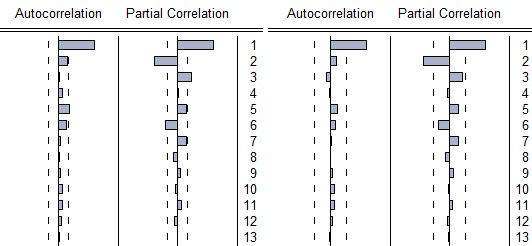
\includegraphics[width=0.75\textwidth]{C:/Users/kc/Downloads/resnls.jpg}
	\caption{Correlogram of residuals resulting from regression of the unconstrained model. The sample is 1871 - 2006 on the left and 1955 - 2006 on the right.}
	\label{correlonls}
\end{figure}
In the correlogram  in figure (\ref{correlonls}) we see that the residuals resulting from the regression of the intrinsic bubble model are certainly not white noise, but they are much less autocorrelated than the residuals resulting from the present-value model. Independently distributed errors is not an assumption of the intrinsic bubble model. 

To assess the statistical significance of the nonlinear term in the intrinsic bubble model, we want to compute a test of the no bubble hypothesis. We can see in the table presented above that in every regression which contained a restricted $\lambda$, the bubble coefficient is significant. When $\lambda$ is not restricted, just using a standard t-test on the hypothesis $c=0$ is to test the significance of the bubble is not correct, since the nonlinear term has two coefficients. $\lambda$ would not be identified in this test. We do not want to assess the significance of that specific coefficient $c$, but of the whole nonlinear term. When $\lambda$ is not restricted, we can compute a F statistic of the no bubble hypothesis as follows: We first estimate the model to obtain the estimate of $\lambda, \widehat{\lambda}$. Then we estimate the model again with the following restriction $\lambda =  \widehat{\lambda}$. We know that $(t_{(d.f.)})^2 = F_{(1,d.f.)}$. So if we square the t statistic of the hypothesis $c=0$, we get the F statistic of the no bubble hypothesis $c=0 ,\lambda =  \widehat{\lambda}$. The nonlinear term is statistically significant at the 1 $\%$ level for every regression shown in table (\ref{NLS}).  
   
The $\lambda$ and $\kappa$ used in table (\ref{NLS})are estimates. To find out whether restricting these parameters makes a significant difference in our model, we perform a likelihood ratio test. We know that $-2(ln(L_0) - ln(L_k)) \sim \chi^2_k$ , where $L_0$ denotes the likelihood of the restricted model and $L_k$ denotes the likelihood of the unrestricted model with $k$ more free parameters. The critical values of the chi-squared distribution are $\chi^2_1(0.05) = 3.84$ and $\chi^2_2(0.05)=5.99$. When we look at the likelihoods of the models obtained by using the subsample, not restricting any parameter does not improve fit significantly compared to restricting one of the parameters. But when we take the whole sample into account, not restricting any parameters does improve fit significantly. Restricting both parameters yields worse results for all models and samples. For the sake of simplicity we continue with the unrestricted model for both samples.

 
We see in table (\ref{NLS}) by looking at the estimates of $c_0$ that a lot of the excessive sensitivity of prices to dividends is absorbed by the nonlinear term. The nonlinear term effectively vanishes when dividend are small, causing the price-dividend ratio and prices to be almost entirely determined by the present-value part of the intrinsic bubble model. Though the present-value model estimates the ratio in table (\ref{sensitivity}) to be over 50, the intrinsic bubble model estimates the ratio to be lower than twenty for small dividends, matching the point estimate $\overline{\kappa}$ reported in table (\ref{point}) much better than the present-value does without the inclusion of the nonlinear term. 

In figure (\ref{pricediv}) we see that before 1955 dividends and prices were relatively calm, both exhibiting a linear trend. In figure (\ref{rationls}) and (\ref{pricenls}) the prices and ratio's estimated by the intrinsic bubble model for both sample periods are plotted. The estimated prices and price-dividend ratio's, $\widehat{P}_t and \widehat{\frac{P_t}{D_t}}$ respectively, are obtained from the following equations 
\begin{eqnarray}
 \widehat{P}_t = D_t(\widehat{c}_0 + \widehat{c}*D_t^{\widehat{\lambda} - 1}) \label{priceestimate}
 \end{eqnarray}
 and 
\begin{eqnarray}
 \widehat{\frac{P_t}{D_t}}= \widehat{c}_0 + \widehat{c}*D_t^{\widehat{\lambda} - 1} \label{ratioestimate}
 \end{eqnarray} 
 where the coefficient have the values estimated by the unrestricted model.  
  The price and ratio estimated by the present-value part of the model, obtained by setting $\widehat{c}=0$, is also included to assess the size of the bubble\footnotemark \footnotetext{The value of $c_0$ estimated by the whole sample, $\widehat{c}_0 = 17.9962$, is used to illustrate the size of the nonlinear term. Had I used the value estimated by the subsample, $\widehat{c}_0 = 12.6979$, the nonlinear term would appear to be even bigger.}.  In the period before 1955 we see that the the models fit rather well. In this period the size of the bubble is very small, what is also reflected in the small differences between the estimations that are made, with and without including the nonlinear term in the model.

\begin{figure}[t]
	\centering
		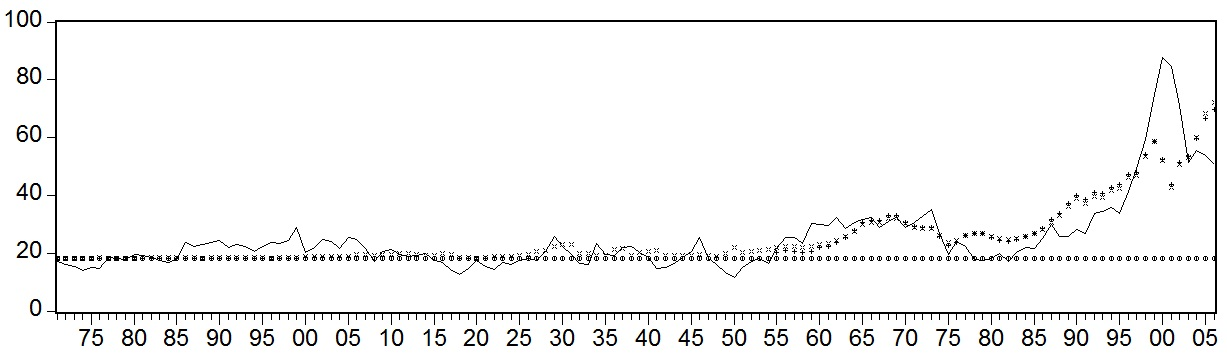
\includegraphics[width=1.1\textwidth]{C:/Users/kc/Downloads/ratiocomparison1.jpg}
	\caption{Plot of price-dividend ratio's. The line represents the actual price-dividend ratio, the 'x signs' the ratio estimated by the intrinsic bubble model using the whole sample, the '$+$ signs' the ratio estimated by the intrinsic bubble model using the subsample and the horizontal line made up by the circles respresent the ratio estimated by the present-value part of the intrinsic bubble model.}
	\label{rationls}
\end{figure}
 
\begin{figure}[h]
	\centering
		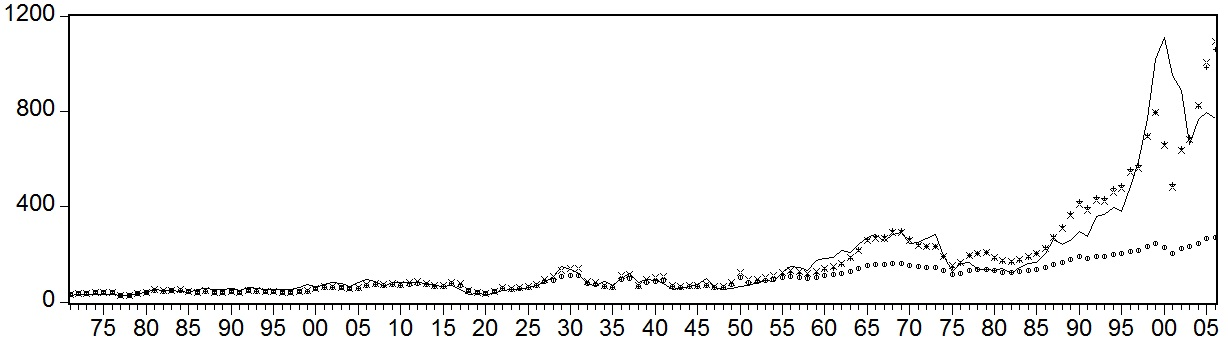
\includegraphics[width=1.1\textwidth]{C:/Users/kc/Downloads/pricecomparison1.jpg}
	\caption{Plot of prices. The line represents the actual pricess, the 'x signs' the prices estimated by the intrinsic bubble model using the whole sample, the '$+$ signs' the prices estimated by the intrinsic bubble model using the subsample and the circles the prices estimated by the present-value part of the intrinsic bubble model.}
	\label{pricenls}
\end{figure}

In figure (\ref{pricediv}) we can see that in the period from 1955 till 1973 prices and dividends suddenly are much higher, breaking with the behaviour they exhibited before 1955. In the period from 1985 till 2006 prices and dividends show extreme behaviour. They grow dramatically. In the plots below we see that the model without the nonlinear term doesn't describe the ratio and the price in these periods very well. The inclusion of the nonlinear term allows the ratio to grow in these high dividend periods and stay high as long as dividends stay high. It also allows the prices to grow exponentially, capturing the explosive movements of prices much better. From 1990 on, the size of the intrinsic bubble is more than half of the predicted price. 

Also noticable in these figures is the fact that the prices and ratio's that are estimated by the intrinsic bubble model using the whole sample are almost indentical to the estimates that are made using the subsample.


To determine whether it is more usefull to only use the data from the subsample or use the data from the whole sample, we look at their predictive powers. The data from 2007 till 2009 are not used in estimating the intrinsic bubble model, so that we can compare these observations with the three-year horizon out-of-sample forecasts. 

\begin{figure}
	\centering
		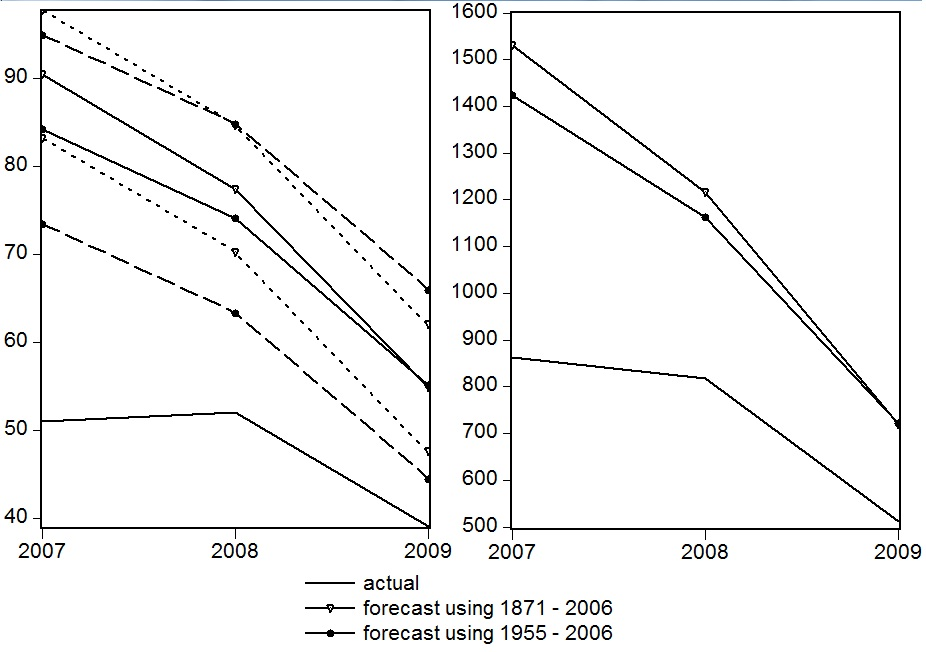
\includegraphics[width=0.7\textwidth]{C:/Users/kc/Downloads/forecasts.jpg}
	\caption{Out-of-sample forecasts for 2007 - 2009. On the left the forecasts of the price-dividend ratio are depicted with the dotted lines representing the standard error margin. On the right the forecasts of prices are depicted.}
	\label{forecasts}
\end{figure}
 
When we look at the plot in figure (\ref{forecasts}) one the left we see that the standard errors produced by using the whole sample are smaller than those produced by the subsample. At the same time we clearly see that the point forecasts made using the whole sample perform worse than the forecasts made by using the subsample. This holds for the point forecasts of prices and price-dividend ratio's. Two conventional measures for evaluating forecasting performance are the root mean squared error, RMSE, which we calculate as follows
\begin{eqnarray}
RMSE = \sqrt{\frac{\sum_{t = 2007}^{2009} (y_t - f(D_t;\widehat{c}_0,\widehat{c},\widehat{\lambda}))^2}{3}} \label{MSE}
\end{eqnarray}
and the mean absolute error, MAE, defined as follows
\begin{eqnarray}
MAE = \frac{\sum_{t = 2007}^{2009} |y_t - f(D_t;\widehat{c}_0,\widehat{c},\widehat{\lambda})|}{3} \label{MAE}
\end{eqnarray}
$y_t$ is the observed ratio or price at time $t$. $f$ is nonlinear predictor function which is (\ref{priceestimate}) in case we forecast prices and (\ref{ratioestimate}) in case we forecast the price-dividend ratio's. 


\begin{table}[h!]
\centering
\begin{tabular}{l | l l| l l }
 &  price & &  ratio &  \\
sample  & RMSE & MAE & RMSE & MAE  \\ \hline
1871 - 2006  & 464.06 & 423.73 &28.54 & 26.83 \\
1955 - 2006 & 398.65 & 371.59 &24.75 & 23.71\\
\end{tabular}
\caption{Measures of forecasting performance}
\label{MSE}
\end{table}

In table (\ref{MSE}) we see that for both measures and series the performance of the forecasts based on the subsample is higher than the performance of the forecasts based on the whole sample. I can not conclude that using a subsample to estimate the model yields significantly better results since the difference in forcasting performance is small and not based on a big forecasting subsample. 

The intrinsic bubble model fits the volatility and the explosive growth of prices much better than the present-value model. Furtermore, it explains  the fact that the price-dividend ratio is not constant. Using a subsample does not produce significantly better result than using the whole sample. The absence of the intrinsic bubble  in the S\&P 500 index is rejected.  



\subsection{nonlinear cointegration}
Finding a long-run nonlinear relation between prices and dividends is empirical evidence consistent with the presence of intrinsic bubbles in the S\&P 500. To test for a nonlinear long-run  price�dividend relationship, we want to test for nonlinear cointegration between prices and dividends. 
 Breitung (2001) shows that  residual-based cointegration tests, like Granger and Hallman's (1991) nonlinear cointegration test, are inconsistent for some classes of nonlinear functions. He suggests a nonparametric cointegration test that uses the rank transformation between two variables and claims it to be more powerfull than parametric cointegration tests if the cointegration relationship is nonlinear. The hypothesis that prices and dividends are  linearly cointegrated is already rejected. Therefore we can savely assume that when Breitung's test gives us evidence for cointegration, it is for nonlinear cointegration. \\

We have assumed prices and dividends to be integrated of order one, since their log transformations are. The null hypothesis that is being tested is that there exist monotonic functions f and g such that 
 \begin{eqnarray}
f(P_t) - g(D_t) = u_t
\end{eqnarray}
where $u_t$ is integrated of order one, which means prices and dividends are not cointegrated. With a rank-based test we don't have to know the specific functions f and g, only that f and g are monotonic functions. Monotonic transformations don't change ranks.
\begin{eqnarray}
R_T (f(P_t)) = R_T (P_t) \notag \\
 R_T (g(D_t)) = R_T (D_t) \notag
\end{eqnarray}
where $R_T(P_t)$ is a function that returns the rank of $P_t$ among $P_{1871},...,P_{2009}$. Prices and dividends are assumed to be integrated of order one, hence random walks. Therefore their rank transformations follow ranked random walks.
When there is a big rank transformation between the series, it seems unlikely that the two series are cointegrated. We assess the size of the transformation by measuring the difference in ranks at each time instant using $\delta_t$.
\begin{eqnarray}
\delta_t = R_T(P_t) - R_T(D_t) \notag
\end{eqnarray}
With this measure we make the following statistics
\begin{eqnarray} 
\kappa_T = T^{-1} \sup_{t} |\delta_t| \notag \\
\xi_T = T^{-3} \sum_{t=1871}^{2009} \delta_t^2 \notag
\end{eqnarray}
These statistics have to be corrected if the considered time series are correlated, which is obviously the case with prices and dividends. To measure the correlation of the ranked series, the following statistic is defined
\begin{eqnarray}
\rho_T^R = \frac{\sum_{t=1872}^{2009} \Delta R_T(P_t)\Delta R_T(D_t)}{\sqrt{(\sum_{t=1872}^{2009} \Delta R_T(P_t)^2)(\sum_{t=1872}^{2009} \Delta R_T(D_t)^2)}} 
\end{eqnarray}
Breitung (2001) shows that for moderate values of correlation between time series, the ranked correlation is  biased downwards in absolute value. With a rank correlation of, $\rho_T^R =0.68$, we have to use the following adjusted test statistics \footnotemark \footnotetext{ See Breitung (2001) for more information on how these statistics are derived.}
\begin{eqnarray}
\kappa_T^{**} =  \frac{\kappa_T}{\widehat{\sigma}_{\Delta \delta} (1-0.174(\rho_T^R)^2)} \label{kappa2} \\
\xi_T^{**} = \frac{\xi_T}{\widehat{\sigma}^2_{\Delta \delta} (1-0.462\rho_T^R)} \label{xi}
\end{eqnarray} 
where $\widehat{\sigma}^2_{\Delta \delta} = T^{-2}\sum_{t=1872}^{2009}(\delta_t - \delta_{t-1} )^2$. We obtain the following statistics $\kappa_T^{**} = 0.3496 $and $ \xi_T^{**} = 0.0144 $. These statistics are both significant at the $5 \%$ level \footnotemark \footnotetext{for critical values, see Breitung (2001).}, so we reject the null hypothesis of no cointegration of prices and dividends. 
One sided testing  is used, since we do not want to investigate a long-run relationship in which prices and dividends are inversely related. These results indicate the existence of  a noninear long-run relation of prices and dividends, which is consistent with the intrinsic bubble model. 

\section{discussion}

This paper provides further empirical evidence that supports the intrinsic bubble model earlier investigated by Froot and Obstfeld (1991) and Ma and Kanas (2004). The failure of the standard present-value model and the improvement in explanatory power of  the behaviour of stock prices and price-dividend ratio's that is yielded by including a nonlinear term in the present-value model is explored. When  a constant discount factor, risk-neutrality of agents and dividends following a geometric random walk is assumed, we  reject the absence of an intrinsic bubble in the S\&P 500 index.  The parameters of the intrinsic bubble for which the no-arbitrage principle would not be violated, are reasonably close to the parameters obtained by performing an unrestricted regression. The nonlinear least squares method used in this paper is explained and an outline of Breitung's (2001) alternative way of testing for cointegration is given. A three-year horizon out-of-sample forecast shows that using a subsample that only includes data after the structural break of dividends in 1955 does improve forecasting powers, but only marginally. The hypothesis of  absence of a linear long-run relation of prices and dividends could not be rejected using a Johansen cointegration test, but the hypothesis of absence of a long-run relation of prices and dividends could be rejected using Breitung's rank-based cointegration test. This can be interpreted as evidence supporting a nonlinear long-run relation of prices and dividends, which is consistent with the intrinsic bubble model.

Although the intrinsic bubble model is much more capable of explaining price behaviour than the standard present-value model, a sidenot on its validity must be made. Beginning in 1990, the S\&P 500 index grows explosively. From 1997 on the intrinsic bubble model really fails to predict and even fit prices. One might questions a models worth, when its only capable of fitting episodes with regular behaviour.
 
 
Economists know that feedback loops play a major role in the dynamics of financial markets, caused by for example agents imitating each other and trend based investment strategies. To reflect this feature in the much used present-value models, speculative exogenous bubbles are often added.
%KIJK HIER NOG FF NAAR!
Obviously, some economists are sceptic about this approach and think of this as seeking refuge in exogenous forces 
so that the present-value model in which prices and fundamentals are linearly related can be kept. In an attempt to explain the boom and busts behaviour of prices through fundamentals, intrinsic bubbles have been suggested as cause. But the problem of not being able to distinguish between misspecification of fundamentals and the presence of bubbles is still present.   

When the inherent weaknesses the bubble approach has in explaining price behaviour are considered, one might ask if a radical new approach is needed. Behavioural economics is a growing field that attacks the main assumption of almost all modern economic theory, namely that agents are fully rational \footnotemark \footnotetext{See for example Akerlof (1991) or for classics see  Simon (1955) and Hayek (1945)}. Personally, I think that the most important future insights about the  dynamics that drive the financial markets will come from a rising field I find particularly appealing, namely complexity economics . Here the economy is not  considered as a system in equilibrium that sometimes has to adjust to an exogenous shock and which is filled with fully rational homogeneous agents, but rather as a constantly evolving self-organizing system filled with interacting heterogeneous agents that are only partly rational and where relations are highly nonlinear through the emergence of feedback loops\footnotemark \footnotetext{For more information on complexity economics see Beinhocker (2006)}. Arthur, Holland, LeBaron, Palmer and Taylor (1997) simulated such a system with agents that made their choices guided by heuristics rather than fully rational expectations. They showed that from systems without those stringent assumptions, boom and busts simply emerged from the dynamics between the interacting agents. This result should urge economists to think about how much potential for future improvement there is for new keyesian economics and encourage them to consider alternative models when trying to explain the dynamics of financial markets.

\section{appendix}

\subsection{Nonlinear least squares data fitting}
If we want to estimate coefficients of a model with a nonlinear specification, we use the method of nonlinear least squares (NLS) estimation. We consider the general nonlinear specification 

\begin{eqnarray}
y = f(\mathbf{x};\theta) + e(\theta) 
\end{eqnarray}
where $y$ is the dependent variable, $f$ a nonlinear function,  $\mathbf{x}\in \mathbb{R}^k$ a vector of explanatory variables, $\theta \in \mathbb{R}^l$ a vector of parameters and $e$ the specification error. Given T observation of $(y,\mathbf{x})$, let


\begin{eqnarray}
\textbf{y} = 
\begin{bmatrix}
y_1 \\ y_2 \\ \vdots \\ y _T \\ 
\end{bmatrix} \text{  ,  } 
f(\mathbf{X}; \theta) = 
\begin{bmatrix} 
f(\mathbf{x_1};\theta) \\
f(\mathbf{x_2};\theta) \\
\vdots \\
f(\mathbf{x_T};\theta) \\
\end{bmatrix} \text{  ,  }
\mathbf{e(\theta)} = 
\begin{bmatrix}
e_1(\theta) \\ e_2(\theta) \\ \vdots \\ e_T(\theta)
\end{bmatrix} 
\end{eqnarray}

We want to find the parameter $\theta$ for our function that best fits the data $(\mathbf{y,X})$. How well our choice of parameters is, is measured by the following formula
\begin{eqnarray}
 S(\theta) = [y - f(\mathbf{X};\theta]'[y - f(\mathbf{X};\theta]  \label{min}
\end{eqnarray}
We want to minimize $S(\theta)$ with respect to $\theta$. A solution $\theta^* \in \mathbb{R}^l$ to this problem must satisfy the first and second order condition of the minimization problem. The first order condition is that the the gradient of (\ref{min}) evaluated at $\theta^*$ must be equal to zero
\begin{eqnarray} 
\frac{dS(\theta)}{d\theta}(\theta^*) = -2 \frac{df(\mathbf{X};\theta)}{d\theta}(\theta^*) [y - f(\mathbf{X};\theta^*]
=  \mathbf{0} \label{foc}
\end{eqnarray}
where 
\begin{eqnarray}
\frac{df(\mathbf{X};\theta)}{d\theta}= 
\begin{bmatrix}
\frac{df(\mathbf{x_1};\theta)}{d\theta} & \frac{df(\mathbf{x_2};\theta)}{d\theta} & \cdots & \frac{df(\mathbf{x_T};\theta)}{d\theta}  \\
\end{bmatrix}
\notag
\end{eqnarray}

Furthermore, to ensure that $S(\theta^*)$ is a minimum and not a maximum, the second order condition of a minimization problem has to be satisfied. The hessian matrix of (\ref{min}), denoted below, evaluated at point $\theta^*$ must be a positive definite matrix.
\begin{eqnarray}   
\frac{d^2S(\theta)}{d\theta d\theta'} =  -2 \frac{d^2f(\mathbf{X};\theta)}{d\theta d\theta'} \cdot [y - f(\mathbf{X};\theta] + 2 \frac{df(\mathbf{X};\theta)}{d\theta} \cdot \frac{df(\mathbf{X};\theta)}{d\theta'} 
 \label{soc}
\end{eqnarray}

The problem with $f$ being nonlinear is that there can be multiple $\theta \in \mathbb{R}$ that satisfy these two conditions. If $f$ were linear, (\ref{foc}) would be a system with l equations and l unknowns. This would give us a unique solution. Furthermore, $\frac{d^2f(\mathbf{X};\theta)}{d\theta d\theta'} $ would be equal to zero and thus $\frac{d^2S(\theta)}{d\theta d\theta'} =  2 \frac{df(\mathbf{X};\theta)}{d\theta} \cdot \frac{df(\mathbf{X};\theta)}{d\theta'} $. This is a sufficient condition for positive definitness.  There is no garantee that there exists a unique solution to this problem if $f$ is nonlinear. This means (\ref{min}) can have multiple local minima. We cannot solve this problem analytically, but we can with an iterative process.
\\
There are a lot of iterative procedures that can lead to a fairly good approximation of the optimal parameter choice. An often used method is the Newton-Raphson algorithm. It uses the second order Taylor expansion of (\ref{min}) around some chosen initial value $\theta_0$
\begin{eqnarray}
S(\theta) \approx S(\theta_0) + (\frac{dS(\theta)}{d\theta}(\theta_0))' (\theta - \theta_0) + \frac{1}{2} (\theta - \theta_0)'\frac{d^2 S(\theta)}{d\theta d\theta'}(\theta_0)(\theta - \theta_0) \label{taylor}
\end{eqnarray}

The first order condition of this expansion with respect to $(\theta)$ is

\begin{eqnarray}
\frac{dS(\theta)}{d\theta}(\theta_0) + \frac{d^2 S(\theta)}{d\theta d\theta'}(\theta_0)(\theta - \theta_0) = 0 \notag
\end{eqnarray}
This can be rewritten as
\begin{eqnarray}
\theta = \theta_0 - (\frac{d^2 S(\theta)}{d\theta d\theta'}(\theta_0))^{-1} \frac{dS(\theta)}{d\theta}(\theta_0)
\end{eqnarray}
So we now know the value $\theta$ that minimizes the taylor expansion . If we now replace $\theta_0$ and $\theta$ with $\theta_i$ and $\theta_{i+1}$ respectively, we get the following algorithm
\begin{eqnarray}
\theta_{i+1} = \theta_i - (\frac{d^2 S(\theta)}{d\theta d\theta'}(\theta_i))^{-1} \frac{dS(\theta)}{d\theta}(\theta_i) \label{algorithm}
\end{eqnarray}
The $(i+1)^{th}$ iterated value $\theta_{i+1}$ is obtained from the value of the previous iteration. 
The downside of this algorithm is that for every iteration the hessian matrix must be positive definite, otherwise it might not be invertible of point in the wrong direction. From (\ref{taylor})(\ref{algorithm}) we can deduce that 
\begin{eqnarray}
S(\theta_{i+1}) - S(\theta_i)\approx   -\frac{1}{2}  (\frac{dS(\theta)}{d\theta}(\theta_i))'  \frac{d^2 S(\theta)}{d\theta d\theta'}(\theta_i)\frac{dS(\theta)}{d\theta}(\theta_i)
\end{eqnarray}
Succesive iterations of $S$ only become smaller if the hessian matrix is positive definite.\\
Sometimes a step length s is added to (\ref{min})
\begin{eqnarray}
\theta_{i+1} = \theta_i - s_i(\frac{d^2 S(\theta)}{d\theta d\theta'}(\theta_i))^{-1} \frac{dS(\theta)}{d\theta}(\theta_i)
\end{eqnarray}
The step length could be determined by minimizing $S(\theta_{i+1})$ with respect to $s_i$. 
\\
An iterative algorithm needs a beginning and an end. The beginning may be some initial value set of values. To minimize the risk of no iteration converging to the global minimum we can generate a lot of  initial values from some distribution and choose the initial value that gives the best result. An algorithm stops when some sort of convergence criteria is met. For example, when 
\begin{eqnarray}
(\theta{i+1} - \theta_i)'(\theta{i+1} - \theta_i) < c
\end{eqnarray}
where $c$ is some small positive pre-determined number. 

\subsection{simulation}

Since we use two relatively small data sets to estimate the parameters of the unrestricted intrinsic bubble model, the estimates made by the nonlinear least squares regression might be biased. The used test statistics might not have the desired distribution when the distributions of the estimates are very skewed or have very fat tails and do not converge to the normal distribution. We can also see whether using the whole sample or the subsample yield has a large impact on the distributions of the estimates. We can evaluate the distribution of the estimates by means of a simulation. We generate 500 time series with the parameters estimated by the unrestricted NLS and see what the distribution is of the estimates of those parameters.  \\

We first construct the log dividends series $\{{d_t}\}_{t=1871}^{2006}$ and $\{{d_t}\}_{t=1955}^{2006}$ as follows 
\begin{eqnarray}
d_t =  d_{t-1} + \epsilon_{t}
\end{eqnarray} 
where the $\epsilon_{t} \sim N(\mu, \sigma_\epsilon^2)$. With each dividends series we generate 500 price series $\{{P_t}\}_{t=1871}^{2006}$ and ${P_{t}}_{t=1955}^{2006}$ as follows
\begin{eqnarray}
P_t = c_0e^{d_t} + ce^{d_t\lambda} + \eta_t
\end{eqnarray}
where $\eta_t = 0.67 \eta_{t-1} -0.5 \eta_{t-2}+ 0.25 \eta_{t-3} $ . In figure (\ref{correlonls}) we can see that these values correspond to the partial autocorrelation coefficients of the residuals estimated by the unrestricted intrinsic bubble model. Since the intrinsic bubble model did not produce white noise residuals but residuals that were autocorrelated, generating residuals as AR(3) processes produces prices series with a higher resemblance to the real prices series.

\begin{table}[h!]
\centering
\begin{tabular}{l|ll}   
parameter & 1871-2006 & 1955-2006 \\ \hline
$\mu$ & 0.016 & 0.020 \\
$\sigma_\epsilon$ & 0.126 & 0.050 \\
$d_0$ & 0.52& 1.72 \\
$c_0$ & 18.0 & 12.7 \\
c & 0.04 & 0.23 \\
$\lambda$ & 3.64 & 3.03 \\
$\sigma_\eta$ 7 & 11 \\  
\end{tabular}
\caption{d}
\label{d}
\end{table}
The parameters used in constructing the dividends series are estimates obtained by regressing log dividends as an random walk with drift.
 
The estimates of these parameters have the following distributions
\begin{figure}[h!]
	\centering
		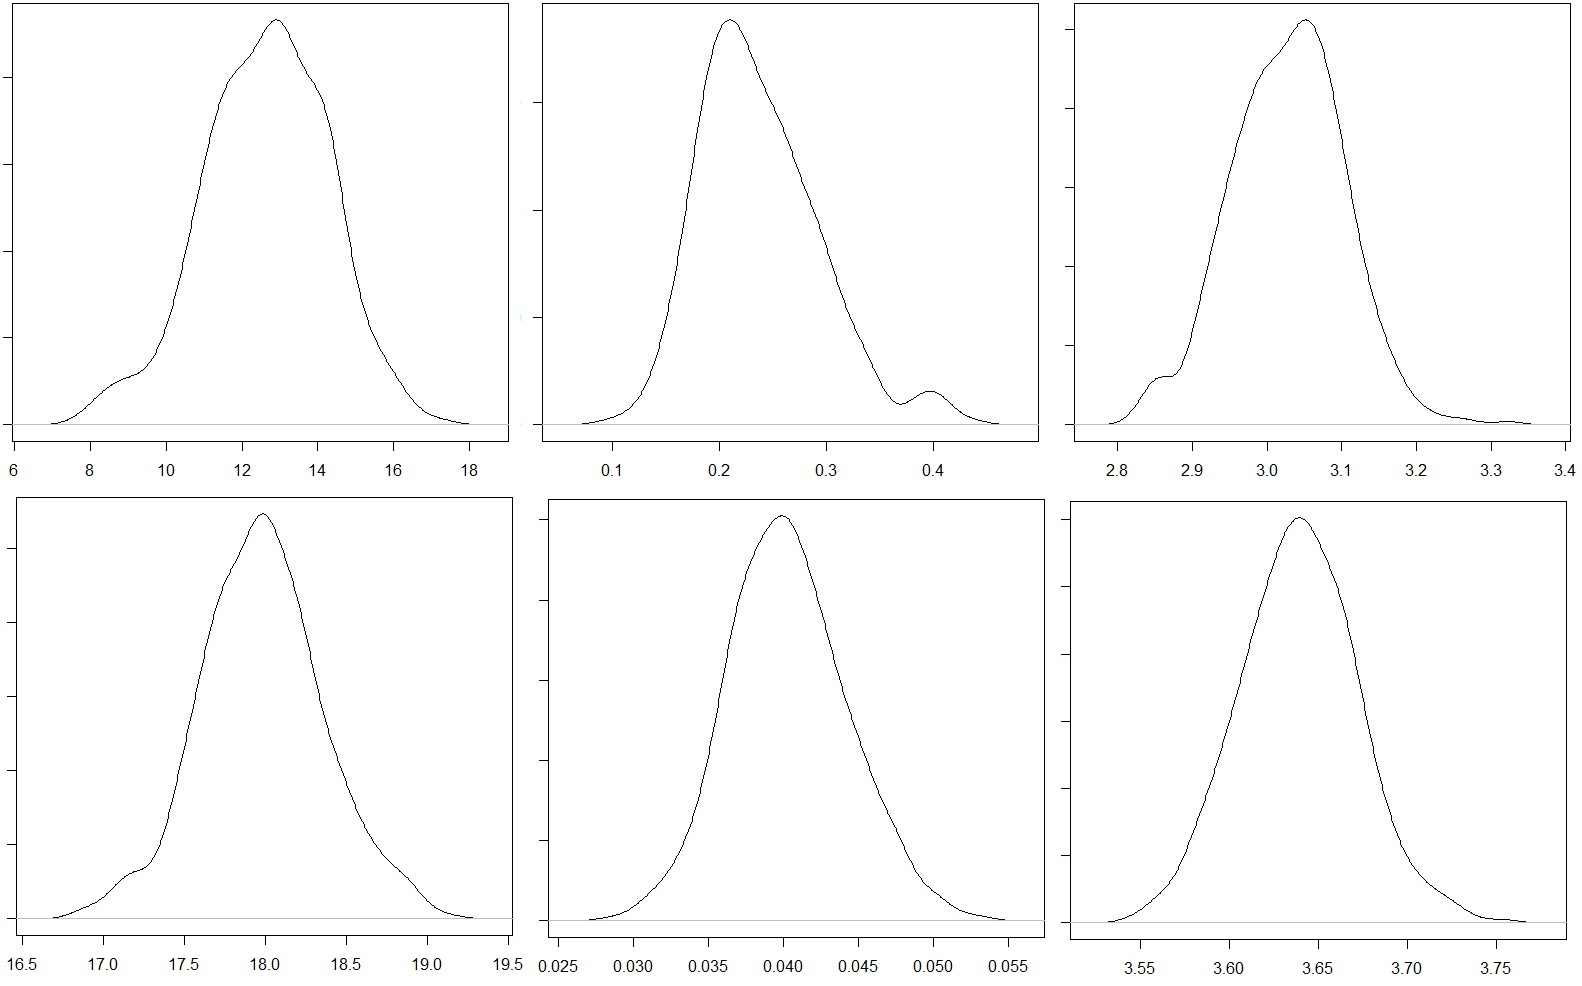
\includegraphics[width=0.9\textwidth]{C:/Users/kc/Downloads/distboth.jpg}
	\caption{Distribution of the estimates made by the intrinsic bubble model. Row one and two plot the distribution of the estimates produced by using the subsample and the whole sample respectively. The first, second and third column show the distribution of the estimates of $c_0, c$ and $\lambda$ respectively. }
	\label{simulation}
\end{figure}

In these plots we see that the distributions of the estimates approximate the normal distribution and are nicely centered around the real values of the parameters. The larger samples yields a less skewed  approximation of the normal distribution, but even with a sample size of 52 the approximation is quite good. 

\subsection{R code}
The R code of the function that returns Breitung's rank-based cointegration test statistics:
\begin{verbatim}
rankcoint <- function(y,x){
   x <- rank(x)
   y <- rank(y)
   n <- length(y)
   dx <- x[2:n]-x[1:n-1]
   dy <- y[2:n]-y[1:n-1]
   Rankrho <- dx%*%dy/sqrt(dx%*%dx*dy%*%dy)
   z <- y-x
   dz<-z[2:n]-z[1:n-1]
   sig<-dz%*%dz/n  
   kap<- max(abs(z))/sqrt(sig*n)
   xi<- z%*%z/sig/n^2;
   kap<- kap/(1-0.174*Rankrho^2)
   xi<-xi/(1-0.462*Rankrho)
return(list(kap=kap,xi=xi))
}
\end{verbatim}
The R code used for simulating the NLS:
\begin{verbatim}
simulate <- function(t,d0,dmu,dsd,error,b){
A <- array(0, dim=c(500,3))
div <- array(0, dim=c(t,1))
div[1] <- d0
#generating dividends 
eps <- rnorm(t-1, mean = dmu, sd = dsd)
for(i in 2:t){
	div[i] <- div[i-1] + eps[i-1]
}
for(j in 1:500){
#adding error that approximates the errors obtained
#unrestricted NLS of the whole sample
ar.sim<-arima.sim(model=list(ar=c(.67,-.5,0.25)),n=t, sd =error)
#constructing price series
P <- b[1]*exp(div) + b[2]*exp(div*b[3]) + ar.sim
beta <- nls(P~ beta1*exp(div) + beta2*exp(div*beta3), 
start=list(beta1 = 15, beta2= 0.1, beta3 = 3), 
control = nls.control(maxiter = 50, minFactor = 1/2048, warnOnly=T),trace=T)
A[j,] <- coef(beta)
}
return(list(b1 = A[,1], b2=A[,2],b3=A[,3]))
}
#then plot densities
sim1955 <- simulate(52,1.72,0.02,0.05,11,c(12.7,0.23,3.03))
plot(density(sim1955$b1), xlim=c(-5,25))
plot(density(sim1955$b2), xlim=c(-2,4))
plot(density(sim1955$b3), xlim=c(0,5))
sim1871 <- simulate(136,0.52,0.0016,0.1257,7,c(18,0.04,3.64))
plot(density(sim1871$b1), xlim=c(-5,25))
plot(density(sim1871$b2), xlim=c(-2,4))
plot(density(sim1871$b3), xlim=c(0,5))
\end{verbatim}

\begin{thebibliography}{breitestes Label}
  \bibitem Akerlof GA. 1991. Procrastination and Obedience. \emph{The American Economic Review}, 2: 1-19.
	\bibitem Blanchard O, Watson MW. 1982. Bubbles, rational expectations and financial markets. \emph{Crises in the Economic and Financial Structure}, Wachtel P(ed.). Lexington Book: Lexington, MA.
	\bibitem Beinhocker ED. 2007. The origin of wealth: The radical remaking of economics and what it means for business and society. Harvard business press: Boston, MA.
\bibitem Bidarkota PV, Dupoyet BV. 2007. Intrinsic bubbles and fat tails in stock prices: a note. \emph{Macroeconomic Dynamics}, 11: 405-422.
	\bibitem Breitung J. 2001. Rank Tests for Nonlinear Cointegration. \emph{ Journal of Business and Economic
Statistics}, 19: 331-340.

	\bibitem Campbell J, Shiller R. 1987. Cointegration and tests of present value models. \emph{Journal
of Political Economy}, 95 : 1062�1088.

	\bibitem Campbell JY, Shiller RJ. 1988a. The dividend-price ratio and the expectations of future dividends and discount factors. \emph{Review of Financial Studies},1: 195-228.
	\bibitem Chen S, Shen C. 2009. Can the nonlinear present value model explain the movement of stock prices? \emph{International Research Journal of Finance and Economics}, 23: 155-170.
	\bibitem De Long JB, Shleifer A, Summers LH, Waldmann RJ. 1990. Noise trader risk in financial markets. \emph{Journal of Political Economy}, 4: 7-3-738.
	  
	\bibitem Diba B, and Grossman H. 1988b. Explosive rational bubbles in stock prices? \emph{American
Economic Review}, 78: 520�530.
	\bibitem Driffill J, Martin S. 1998. Intrinsic bubbles and regime-switching. \emph{Journal of Monetary
Economics}, 42: 357�373.
	\bibitem Evans G. 1991. Pitfalls in testing for explosive bubbles in asset prices. \emph{American Economic
Review}, 31: 922�930.
\bibitem Flood R, P. Garber. 1980. Market Fundamentals versus Price-Level Bubbles, the First
Tests. \emph{ Journal of Political Economy}, 88:745-770.

	\bibitem Flood R, and Hodrick R. 1986. Asset price volatility, bubbles and process switching. \emph{
Journal of Finance}, 41: 831�842.

	\bibitem Froot K, Obstfeld M. 1991. Intrinsic bubbles: The case of stock prices. \emph{American Economic Review}, 81: 1189-1214.
	
	\bibitem G�rkaynak RS. 2008. Econometric tests of asset price bubbles: taking stock. \emph{Journal of Economic Surveys},
 22(1): 166-186.
 \bibitem Hayek FA. 1945. The use of knowledge in Society. \emph{The American Economic Review}, 4: 519-530.
 \bibitem LeRoy S, Porter R. 1981. The present-value relation: tests based on implied variance
bounds. \emph{Econometrica}, 49: 555�574.
 \bibitem Lucas Jr, Robert E. 1978 Asset prices in an exchange economy. \emph{Econometrica}, 46: 1429�
1445.
 
 \bibitem Ma Y, Kanas A. 2004. Intrinsic bubbles revisited: evidence from nonlinear cointegration and forecasting. \emph{Journal of Forecasting}, 23: 237�250.
 
 \bibitem Shiller R. 1981. Do Stock Prices Move Too Much to be Justified by Subsequent Changes in
Dividends? \emph{American Economic Review}, 71: 421-436.
\bibitem Simon HA. 1955. A behavioural model of rational choice. \emph{The Quarterly Journal of Economics}, 1: 99-118. 

 \bibitem West KD. 1987. A Specification Test for Speculative Bubbles. \emph{ Quarterly Journal of
Economics}, 102: 553-580.

 \bibitem  West KD. 1988. Dividend Innovations and Stock Price Volatility. \emph{Econometrica}, 56: 37-61,
 
\end{thebibliography}

% beinhocker , hayek, herbert simmons, chen, bidarkota dupoyet invoegen. vervolgens  code klaarmaken en verhaal fatsoeneren 
 
\end{document}